% !Mode:: "TeX:UTF-8"
% !TEX program  = xelatex
\documentclass[a4paper]{article}
\usepackage{amsmath}
\usepackage{amssymb}
\usepackage{ctex}
\usepackage{graphicx}
%\usepackage{braket}
\usepackage[european]{circuitikz}
\usepackage{multirow}
\usepackage{geometry}
\usepackage{float}
\geometry{left=2.5cm,right=2.5cm,bottom=2.5cm,top=2.5cm}
\title{物理化学实验: 电动势的测定及其应用}
\author{薛明怡\quad 151250177\quad 化学化工学院}
\date{\today}
\begin{document}
\maketitle
%%\tableofcontents
%%\bibliographystyle{unsrt}
\section{实验目的}
\begin{enumerate}
\item 掌握银电极, 银--氯化银电极的制备方法.
\item 掌握电位差计的使用方法.
\item 掌握对消法测定电池电动势.
\item 掌握可逆电池电动势的应用.
\item 对实验结果进行讨论并设计拓展实验.
\end{enumerate}
\section{实验原理}
\subsection{原电池}
原电池是由两个``半电池''组成, 每一个半电池中包含一个电极和
相应的电解质溶液. 不同的半电池可以组成各种各样的原电池.
\par
\subsection{电池电动势}
电池电动势为组成该电池的两个半电池的电极电势的代数和. 
已知一个半电池的电极电势, 通过测定电动势, 即可求得另一半电池的电极电势.
电极电势包括界面电势差(扩散双电层模型), 接触电势和液接电势等.
\subsection{双液电池和盐桥}
如果两个半电池的电极反应所涉及的反应离子不能由同一种电解质提供, 
而需要用到两种电解质溶液时, 需要将两种电解质溶液隔开(通常使用素瓷烧杯或盐桥), 
这种电池称为双液化学电池.
\par 
盐桥是充满正, 负离子迁移数十分接近的高浓度电解质通道, 能有效减小
液接电势. $1\% - 2\%$琼脂的饱和$KCl$盐桥可以消除液接电势, 
其原因是$K^{+}$和$Cl^{-}$的迁移数十分接近, 而$KCl$的浓度远大于
其他电解质, 扩散和迁移主要由$K^{+}$和$Cl^{-}$完成, 因此液接电势的
数值可以降低到$1 - 2mV$, 在一般的电动势测量中, 这一微小数值可忽略不计.
\subsection{对消法}
如果选用伏特计测定电池电动势, 电路中存在的电流和内电阻会产生内电势降, 
测得的只能是两电极的端电压, 数值小于电池电动势. 所以用伏特计无法测出电动势. 
对消法测定电动势使用的仪器为电位差计, 在电流接近0的条件下测定(可逆条件), 
如下图:
\begin{figure}[H]
	\centering
	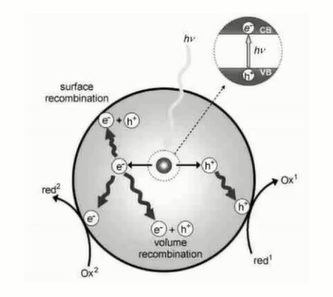
\includegraphics[width = 0.30\paperwidth]{fig/principle.png}
	\caption{对消法测定电池电动势原理}\label{wf}
\end{figure}
\begin{equation}
	\centering
	\begin{aligned}
		E &= (R_{0} + R_{i})I\\
		U &= R_{0}I\\
		\frac{U}{E} &= \frac{R_{0}}{R_{0}+R_{i}}\\
		R_{0}&\to \infty, E\approx U\\
		E_{x} &= E_{s.c}\frac{AC}{AH}\\
	\end{aligned}
\end{equation}
\subsection{电动势测定的应用}
\begin{itemize}
	\item 求难溶盐的活度积.
	\item pH的测定.
	\item 求电解质溶液的平均活度因子.
	\item 离子选择性电极和化学传感器.
	\item 细胞膜与膜电势.
\end{itemize}
在本实验中需要求难溶盐的活度积和测定未知溶液的pH.
\begin{equation}
	\centering
	\begin{aligned}
		E &= E^{\theta} - \frac{RT}{F}ln\frac{1}{a_{Ag^{+}}\cdot a_{Cl^{-}}}\\
		E^{\theta} &= \frac{RT}{F}ln\frac{1}{K_{sp}}\\
		lgK_{sp} &= lg(a_{Ag^{+}}\cdot a_{Cl^{-}}) - \frac{EF}{2.303RT}\\
		\phi_{} &= \phi_{C_{12}H_{10}O_{4}}^{\theta} - \frac{RT}{2F}ln(\frac{a_{C_{6}H_{6}O_{2}}}{a_{C_{6}H_{4}O_{2}}a_{H^{2}}^{2}})\\
			& = \phi_{C_{12}H_{10}O_{4}}^{\theta} - \frac{2.303RT}{F}pH\\
		pH &= \frac{\phi_{C_{12}H_{10}O_{4}}^{\theta}-E-\phi_{Hg,Hg_{2}Cl_{2}}}{2.303RT/F}
	\end{aligned}
\end{equation}
\section{仪器与药品}
\begin{enumerate}
    \item \textbf{仪器:} 数字电位差综合测试仪, 韦斯顿标准电池, 稳流电源, 铁架台, 去离子水洗瓶, 废液烧杯, 
    $50mL$烧杯2只, $10mL$烧杯4只, 盐桥支架, 电阻炉, U型管, 磁力搅拌加热器.
    \item \textbf{药品:} 盐桥液, $Ag$电极$3$支, $Pt$电极$2$支, 饱和甘汞电极, 电池盒, 
	饱和$KCl$溶液, 醌氢醌固体, 未知pH溶液, $0.01mol/L~KCl$溶液, $0.1mol/L~HCl$溶液, 
	$1mol/L~HCl$溶液, $0.01mol/L~AgNO_{3}$溶液, $0.1mol/L~AgNO_{3}$溶液, 镀银液.
\end{enumerate}
\section{实验步骤}
\subsection{制备电极}
\subsubsection{制备银电极}
\begin{itemize}
	\item 用细砂纸将三支银电极打磨光亮, 用去离子水冲洗, 擦干备用.
	\item 将一支银电极和一支铂电极固定到铁架台上, 在$10mL$小烧杯中加入
	约$8mL$镀银液, 将两支电极浸入镀银液中.
	\item 银电极接入稳流电源负极, 铂电极接入正极.
	\item 打开稳流电源开关, 调节电流至$2mA$, 镀银$40min$.
	\item 同法电镀另两支银电极, 放入去离子水中保存.
	\item 为了减少表面电势差的影响, 使用前银电极银棒处接触几秒钟.
\end{itemize}
\subsubsection{制备银-氯化银电极}
\begin{itemize}
	\item 电解液为$1mol/L~HCl$溶液, 新制银电极接入正极, 铂电极接入负极
	(与制备银电极相反).
	\item 打开稳流开关, 调节电流约为$2mA$, 通电$15min$.
\end{itemize}
\subsection{制备盐桥}
\begin{itemize}
	\item 打开电阻炉和磁力搅拌加热器开关, 加热U型管清洗液, 融化盐桥液.
	\item 用镊子从热水中取出U型管, 倒掉管内液体, 立即用滴管从一端加入
	融化的盐桥液, 一次性加满, 中间不能有气泡, 否则需要重新灌制.
	\item 制备好的盐桥斜靠在盐桥支架上自然冷却, 同法再灌制$3-4$根盐桥.
	\item 待盐桥冷却后, 向U型管两端补加少量盐桥液填平.
\end{itemize}
\subsection{校正电位差计}
\begin{itemize}
	\item 打开数值电位差综合测试仪开关.
	\item 若用内标法校正, 调节电位指示为1V. 将``测量选择''旋钮转至``内标''档,
	按``归零''键将``检零指示''调至零, 将``测量选择''转至``断''位置.
	\item 若用外标法校正, 需要使用标准电池. 将综合测试仪``外标+'' ``外标-''接线口
	分别连上标准电池正负极, 根据标准电池电势随温度变化关系式计算出当前温度下电动势数值.
	调节``电位指示''为对应电动势数值, 将``测量选择''旋钮转至``外标'', 按``归零''键, 
	将``测量选择''转至``断''位置.
\end{itemize}
\subsection{测量电池电动势}
\begin{itemize}
	\item 银电极和甘汞电极构成电池的电动势数值.
	检查甘汞电极内是否存在气泡, 特别是转角处, 若有则轻敲管壁赶走气泡; 电极内
	液面应到支管液面加液口处, 若液体不足, 可用滴管从加液口加入饱和$KCl$溶液.\\
	将盛有约$5mL$饱和$KCl$溶液的$10mL$烧杯放入电池盒中, 插入饱和甘汞电极, 接入测试仪``测量-''插口; 
	将盛有约$5mL~0.01mol/L~AgNO_{3}$溶液的$10mL$烧杯放入电池盒中, 插入银电极, 接入测试仪``测量+''插口. \\
	将电位指示调至$0.5V$左右, 测量选择调至``测量''再转回``断'', 
	根据``测量''状态时``检零指示''显示的零点差值调节``电位指示''数值, 实际值约等于当前``电位指示''值减去``检零指示''值.
	然后调至``测量''再转回``断'', 再进一步调节``电位指示'', 直至校零指示为0. 此时``电位指示''为该电池电动势.\\
	$Hg(s)|Hg_{2}Cl_{2}(s)|$饱和$KCl$溶液$||AgNO_{3}(0.100mol\cdot L^{-1})|Ag(s)$
	\item 更换电极溶液, 将一支新制银电极插入$0.01mol/L~AgNO_{3}$溶液的$10mL$烧杯中, 
	在$0.01mol/L~KCl$溶液的$10mL$烧杯中滴加$2$滴$0.1mol/L~AgNO_{3}$溶液, 边滴边搅拌, 插入
	另一支新制银电极, 在两烧杯溶液中插入一根新盐桥. $AgNO_{3}$溶液中的银电极接入``测量+'', 
	$KCl$溶液中的银电极接入``测量-''. 按上述步骤操作测量电极电动势. \\
	$Ag(s)|$饱和$AgCl$的$KCl(0.010mol\cdot L^{-1})$溶液$||AgNO_{3}(0.010mol\cdot L^{-1})|Ag(s)$
	\item 醌氢醌电极制备时往未知pH溶液中加入少量醌氢醌固体, 搅拌后放置几分钟达到溶解平衡, 
	插入铂电极. 在两烧杯溶液中插入一根新盐桥, 铂电极接``测量+'', 甘汞电极接``测量-''. 测量此电极电动势.\\
	$Hg(s)|Hg_{2}Cl_{2}(s)|$饱和$KCl$溶液$||$饱和醌氢醌的未知$pH$溶液$|Pt(s)$
	\item 将银电极插入$0.1mol/L~AgNO_{3}$溶液接``测量+'', 银--氯化银电极插入$0.1mol/L~HCl$溶液接``测量-'', 
	插入盐桥. 测量此电极电动势.\\
	$Ag(s)|AgCl(s)|HCl(0.100mol\cdot L^{-1})$溶液$||AgNO_{3}(0.100mol\cdot L^{-1})|Ag(s)$
	\item 测试完毕, 盐桥放入电阻炉上盛去离子水的烧杯中, 加热煮沸清洗, 中间换几次水. 
	清洗其他仪器并复原.
\end{itemize}
\section{注意事项}
\begin{enumerate}
	\item 盐桥的制备过程.
	\item 保证测定过程中电流基本为0.
	\item 测量速度要快.
	\item 正负极不要接反.
\end{enumerate}
\section{数据处理}

% \section{拓展实验}
\newpage
\section{思考与讨论}
\begin{enumerate}
	\item 将电池放置一段时间看看电动势发生什么变化?\\
	(1) 如果是金属-金属难溶盐电极, 例如新制银-氯化银电极, 则将电极放置一段时间后, 
	银电极可能陈化生成氧化银, 导致电极的构成发生变化. (2) 如果是金属-金属盐溶液电极, 
	则放置时间过长会导致溶液中金属离子浓度产生变化, 浓度增大电势升高, 浓度减小
	电势降低. (3) 如果电池在防止过程中有电流通过, 则可能造成电极极化, 
	以及由于电池充放电造成的电极构成变化.
	\item 测量电池的电极电动势需要哪些条件? 误差有哪些?\\
	测量条件: 电极中几乎没有电流通过, 不产生极化, 接近于热力学平衡态没有动力学阻碍.\\
	误差: (1) 仪器误差. (2) 溶液配制造成的浓度误差. (3) 在电极制备过程中, 由于电流太大造成
	新制银电极层疏松易被空气中氧气氧化为$Ag_{2}O$.
	\item 在拓展实验中, 甘汞电极溶液为饱和$KCl$溶液, 由于电极电势为$\phi_{Hg|Hg_{2}Cl_{2}} 
	= \phi^{\theta}_{Hg|Hg_{2}Cl_{2}} + \frac{RT}{2F}\ln\frac{1}{a(Cl^{-})^{2}}$, 随温度的升高, 
	$KCl$溶解度增大导致$Cl^{-}$升高, $\ln\frac{1}{a(Cl^{-})^{2}}$造成的电极电势的下降超过了由于温度升高
	造成的$\frac{RT}{2F}$的升高, 因此拓展实验中不同温度下饱和$KCl$溶液甘汞电极的电势下降.
	\item 对消法测定电池电动势的装置中, 电位差计, 工作电源, 标准电池
	及检流计各起什么作用?\\
	电位差计包括了一个可变电阻$R$, 一个固定电阻$R_{n}$, 一个带滑动头的固定电阻$R_{a}$, 
	转换开关和一些导线, 构成了除工作电源, 标准电池, 检流计以外对消法测定电动势装置.
	工作电源是为了构成工作电路, 在固定电阻上产生电位降, 用作对消电动势.  标准电池是为了
	校准工作电流, 通过在$R_{n}$上产生电位降与标准电池对消来确定工作电流大小. 检流计是为了
	检测电路中是否存在电流, 即待测电动势与外接电动势是否对消, 符合电动势测定时外电路电流为0的条件.
	\item 如果根据下述电池安排实验测定银电极电极电势, 实验中会出现什么现象? 如何纠正? \\
	$Ag|AgNO_{3}(a = 1)||H^{+}(a=1)|H_{2}(p^{\theta})|Pt(s)$\\
	实验中会出现检流计一直偏转现象. 对于一个电池, 通常用电势低的电极作负极, 电势高的电极作正极.
	在本题中给出的电池, 氢电极为正极, 电势电极为0, 银电极为负极, 电极电势为$0.7991V$, 照这样
	接入电位差计中, 外接电动势就与之方向相同, 无法产生对消, 造成电池一直处于放电状态. \\
	解决方式: 将正负极对调.
	\item 测量过程中, 若检流计光点总是往一个方向偏转, 可能是哪些原因引起?\\
	检流计光点总是往一个方向偏转说明检测电路中始终有电流存在, 可能原因有:
	(1) 工作电源没有打开或电压过低. 
	(2) 电池正负极接反. 
	(3) 测量线路中出现接触不良或短路现象.
	(4) 电池电动势超出了电位差计检测范围.
	(5) 调节值还处于远偏离电池电动势的状态.
	\item 测量电势为何要选用盐桥? 选择"盐桥液"应该注意什么问题?\\
	选用盐桥是为了减小液接电势. 盐桥液要求: 
	(1) 高浓度的盐溶液.
	(2) 正负离子迁移速率相近.
	(3) 不与两端电池溶液发生反应.
	(4) 常加入琼胶做胶凝剂, 由于琼胶含有高蛋白所以要新鲜配制.
	\item 用$Zn(Hg)$与$Cu$组成电池, 有人认为锌表面有汞, 因而铜为负极, 汞为正极. 
	请分析此结论是否正确?\\
	不对. 从金属活泼性看, $Zn>Cu>Hg$, 放电顺序应为Zn, Cu, Hg. 在$Zn(Hg)$中, $Zn$实际上
	溶于Hg形成了饱和溶液, 活度为1, 在$Zn(Hg)$表面上发生反应的还是Zn, 作为负极, 而铜作为正极.\\
	在$Zn(Hg)$中加入$Hg$是因为通常$Zn$棒中含有其他金属杂质, 在溶液中本身会形成微电池, 产生氢气, 
	因而不能直接用作电极. 而$Zn$溶于$Hg$形成$Zn(Hg)$, 活度仍为1, 但是由于$H_{2}$在$Hg$上超电势
	较大, 不易析出, 在实验条件下较易达到平衡.
\end{enumerate}
% \newpage
% \section{原始数据记录}
% \begin{table}[H]
% 	\caption{电动势测定数据记录}
% 	\begin{center}
% 		\begin{tabular}{l|l|l}
% 			\hline
% 			电池\quad\quad& 电动势/V \quad\quad\quad\quad& 测定温度 $^\circ$C\quad\quad\\
% 			\hline
% 			1 &	&	\\
% 			&	&	\\
% 			\hline
% 			2 &	&	\\
% 			&	&	\\
% 			\hline
% 			3 &	&	\\
% 			&	&	\\
% 			\hline
% 			4 &	&	\\
% 			&	&	\\
% 			\hline
% 		 \end{tabular}
% 	\end{center}
% \end{table}
%%\bibliography{ref}
\end{document}